\documentclass[12pt,german]{article}
\usepackage{listings}
%\usepackage[utf8]{inputenc}
\usepackage{inputenc}
\usepackage{graphicx}
\usepackage{float}
\usepackage{array}
\usepackage{pdfpages}

\lstset{
extendedchars=\true,
language=JAVA,
numbers=left, 
numberstyle=\footnotesize, 
%inputencoding=utf8,
%basicstyle=\ttfamily,
%basicstyle=\ttfamily\fontsize{8}{8},
%commentstyle=\ttfamily\fontsize{8}{8},
basicstyle=\tiny;
columns=fullflexible,
%xleftmargin=5pt,
frame=single,
breaklines=true,
postbreak=\mbox{{$\hookrightarrow$}\space},
}
\renewcommand{\thesubsubsection}{\alph{subsubsection} )}
%\renewcommand{\thesubsubsection}{\thesubsection.\alph{subsubsection} )}

\setcounter{section}{1}

\begin{document}

\title{Übungsaufgaben II, SBV1 }
\author{Lukas Fiel, Lisa Panholzer}
\maketitle


\newpage
\section{Übungsaufgaben III}
\subsection{Resampling und Interpolation}
\subsubsection{Implementierung Resampling}


hier könnte Ihr text stehen
\begin{figure}[H]
	\centering
	%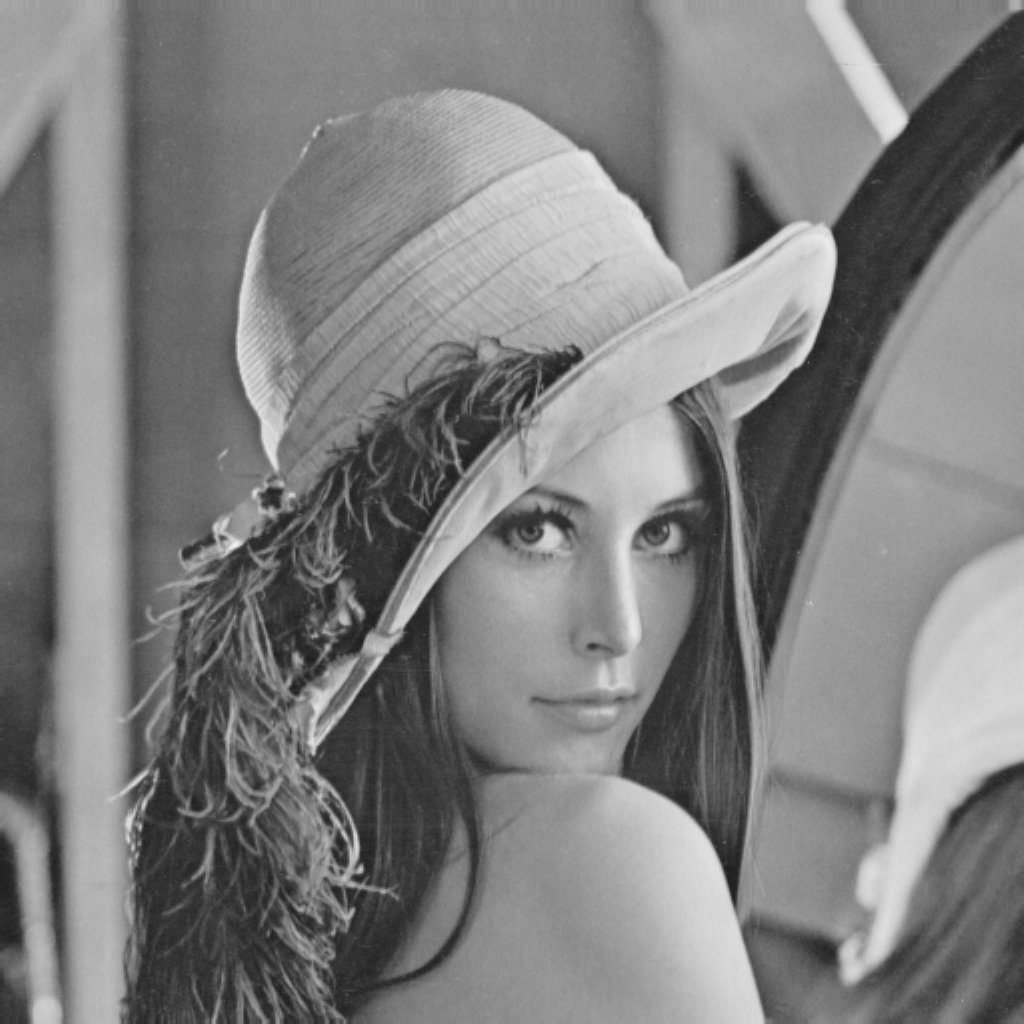
\includegraphics[width=7cm]{images/bilineare-interpolation-final/bip-scaled-2.jpg}
	\caption{Resampling anhand bilinearer Interpolation und Skalierung um Faktor 2.0}
	\label{fig:resultResamplingBilinearInterpolation-2.0}
\end{figure}


\begin{table}[H]
  \centering
  \begin{tabular}{| l | c | c | c | c | c |}
	\hline
	Datensätze & Abstract & Dictionary & Facebook & Google & Witz \\ 
    \hline
    Abstract &
  %  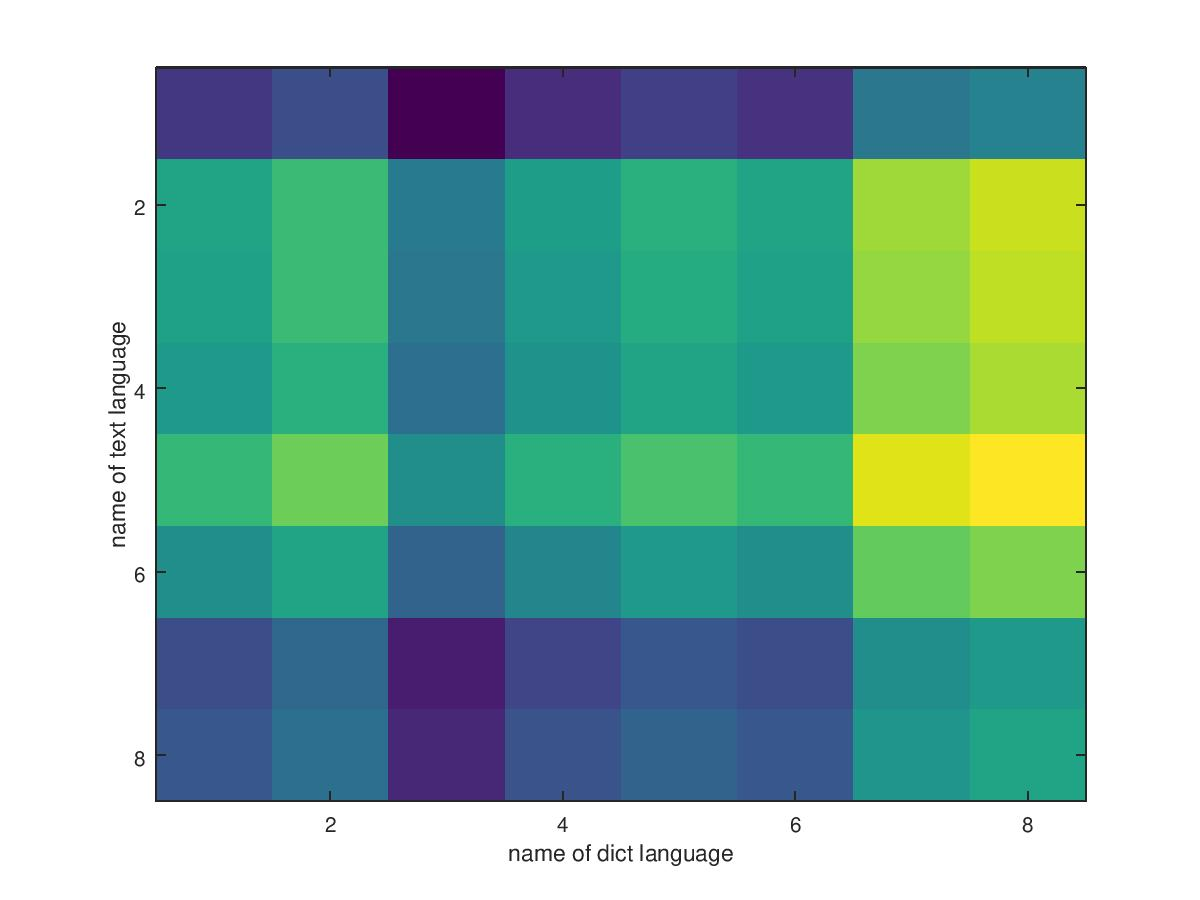
\includegraphics[width=2.5cm]{../images/abstractData/abstractData.jpg} &
  %  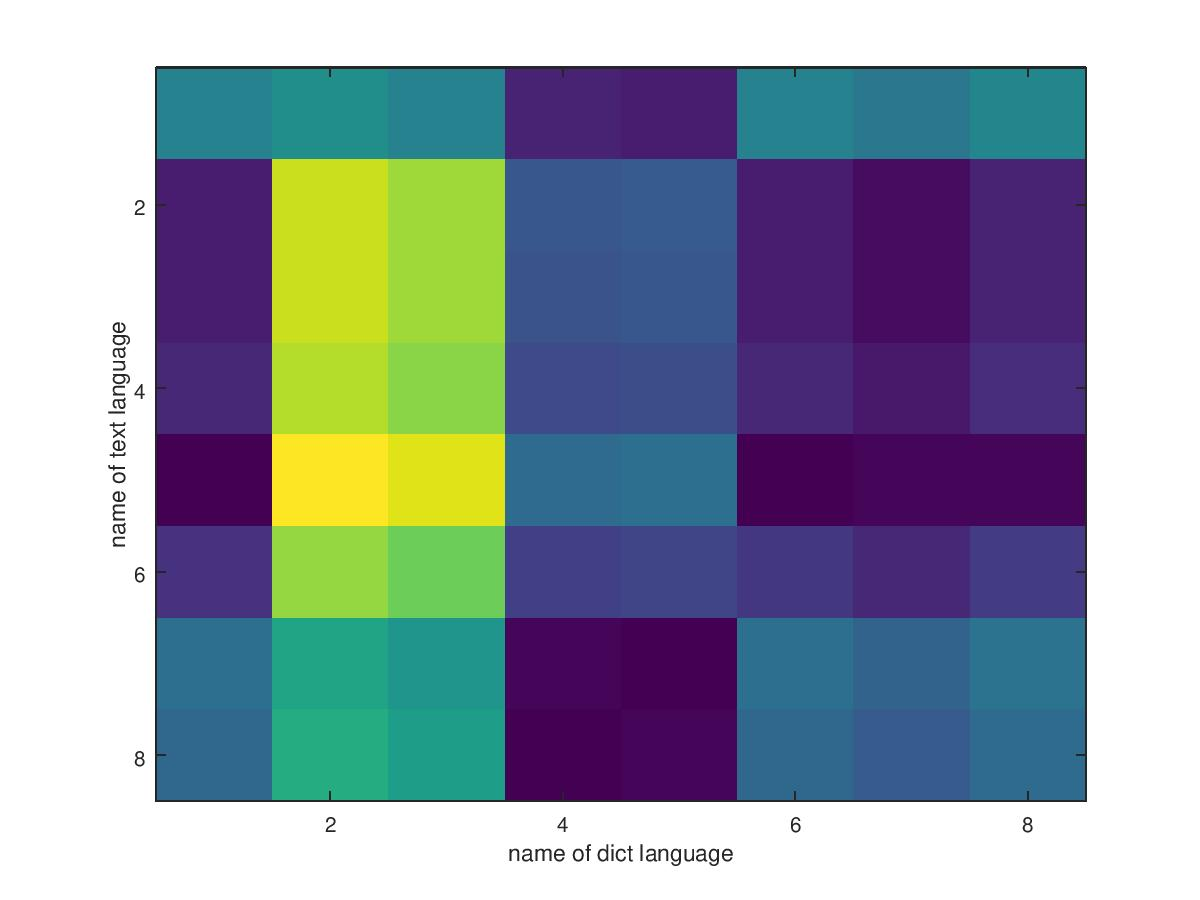
\includegraphics[width=2.5cm]{../images/abstractData/dictData.jpg} &
  %  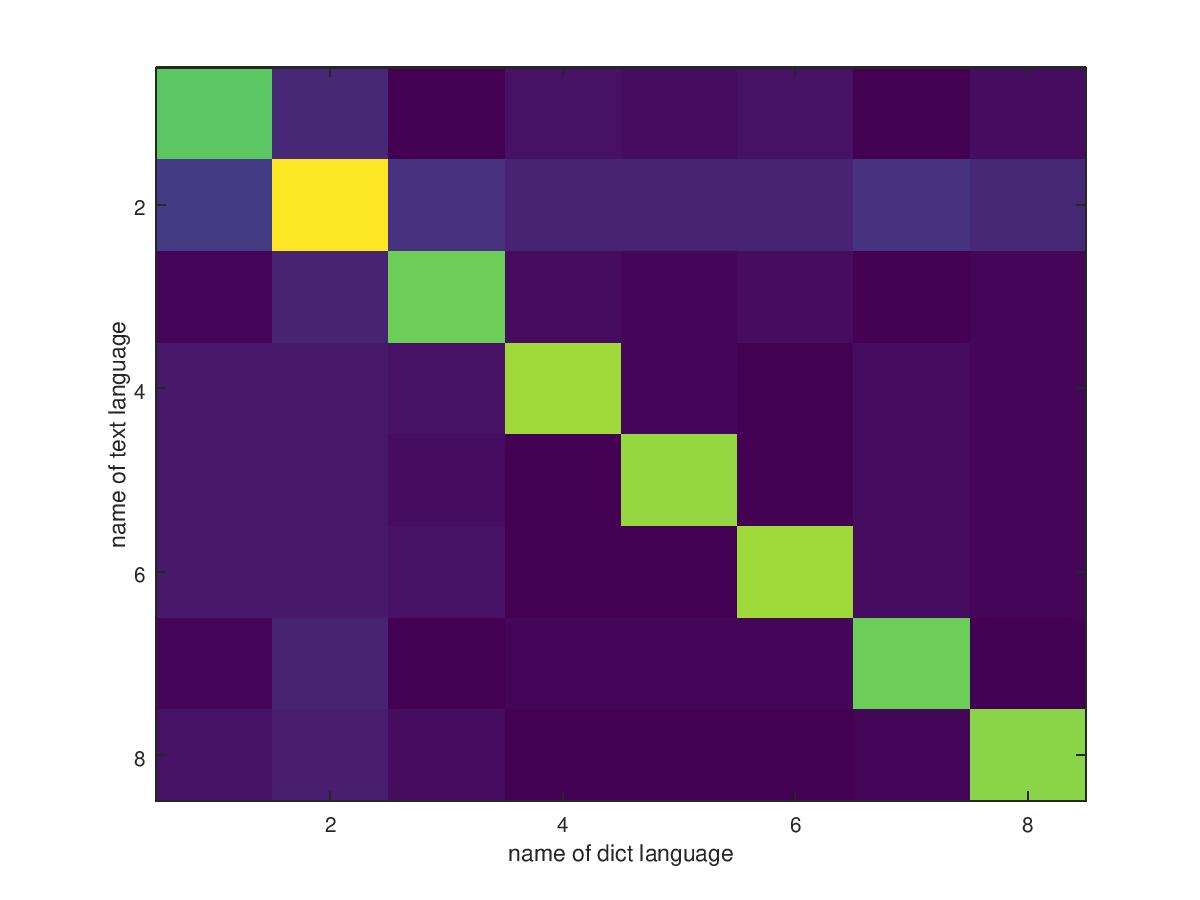
\includegraphics[width=2.5cm]{../images/abstractData/facebookData.jpg} &
  %  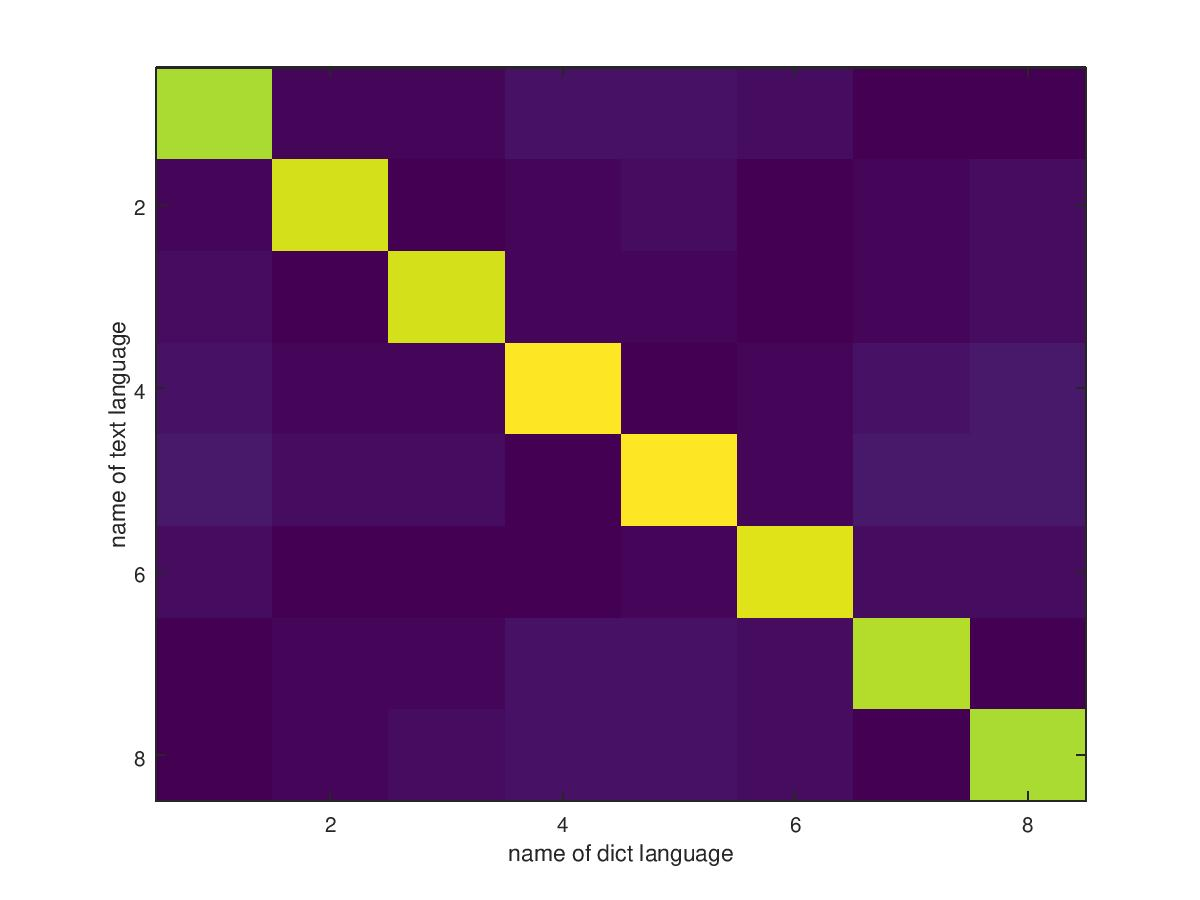
\includegraphics[width=2.5cm]{../images/abstractData/googleData.jpg} &
  %  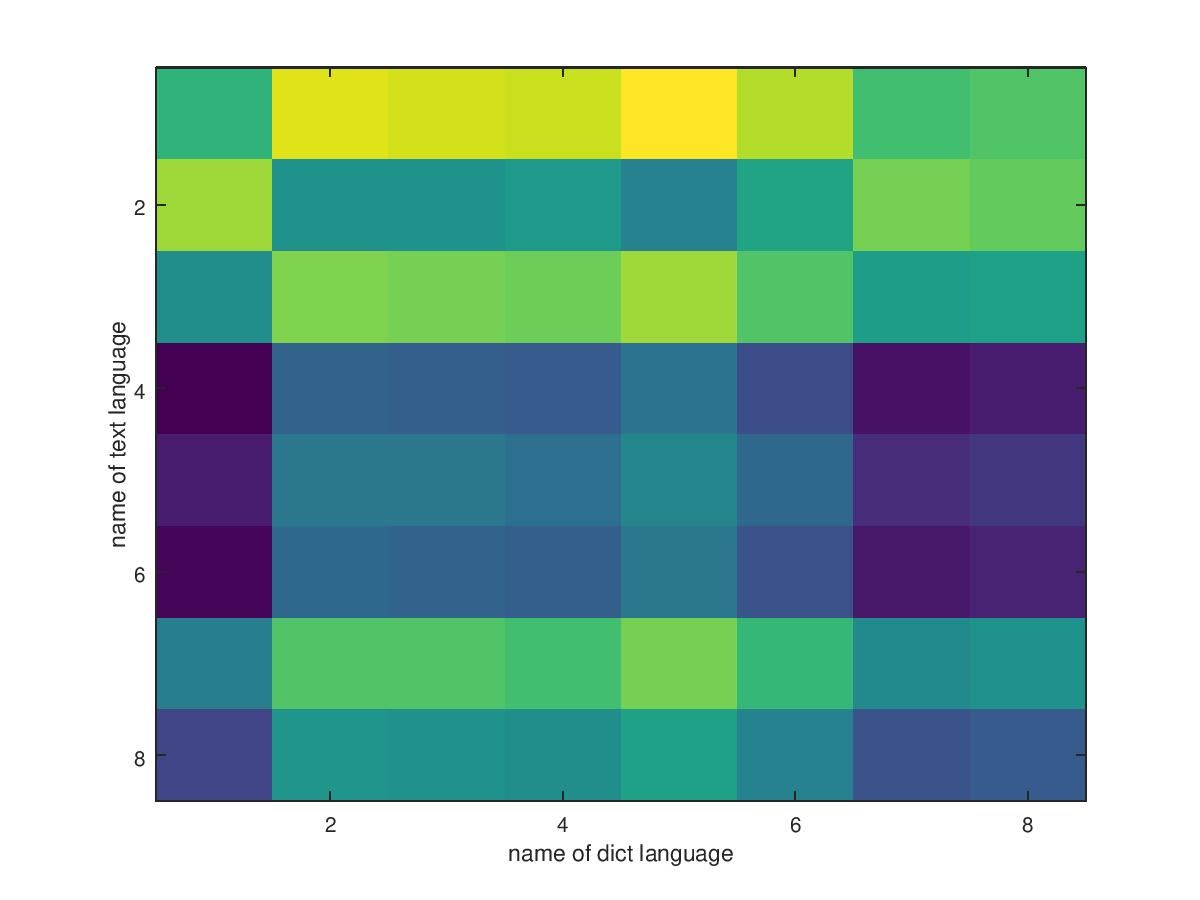
\includegraphics[width=2.5cm]{../images/abstractData/witzData.jpg} \\
  %  \hline
    
  \end{tabular}
  \caption{Auswertung der Datensätze}
  \label{tab:datenAuswertungText}
\end{table}

\newpage
%%\lstinputlisting[frame=single,language=MATLAB,breaklines=true,caption = Octave Script zur Darstellung der einzelnen Kompressionsraten.]{../calculateZipMatrix.m}
%%\label{fig: calculateMatrixOctaveCode}



\end{document}
